\documentclass[border=2pt]{standalone}
\usepackage{amsmath}
\usepackage[dvipsnames]{xcolor}
\usepackage{float}
\usepackage{tikz}
\usepackage{pgfplots}
\usetikzlibrary{calc}
\usetikzlibrary{intersections}
\usetikzlibrary{positioning}
\usetikzlibrary{graphs}
\usetikzlibrary{backgrounds}
\usetikzlibrary{plotmarks}
\usetikzlibrary{shapes.geometric}
\usetikzlibrary{shapes.arrows}
\usepackage{graphicx}
\pgfplotsset{compat=1.18}

\begin{document}
\definecolor{bluee}{RGB}{68,114,196}

\begin{tikzpicture}[font=\footnotesize]
\draw[black!50,fill=black!10](0.19,0)
--++(90:4)coordinate(GAS)
--++(0:4.87)--++(270:2.23)--++(180:0.1)
--++(90:2.13)--++(180:4.67)--++(270:3.91);
%
\draw[fill=black!10]
(0,0)--(0.3,0)--++(43:0.32)--++
(90:1.55)--++(0:0.2)--++(90:0.5)coordinate(P)
--++(0:0.14)--++(270:0.5)--++(0:1.46)
--++(90:0.3)coordinate(SP1)
--++(115:0.5) %kosa
--++(90:0.52)coordinate(PEEP)
--++(0:0.7)--++(270:0.6)
--++(315:0.95)--++(0:0.35)coordinate(A)
--++(45:0.1)--++(0:0.4)
--++(325:0.12)--++(0:3)
--++(90:0.15)--++(180:0.57)coordinate(APL)
--++(90:0.60)coordinate(AAPL)--++(0:0.57)
--++(90:1.23)coordinate(V)
--++(135:0.3)--++(90:0.3)coordinate(V1)
--++(0:2.3)coordinate(V2)
--++(270:0.2)coordinate(V22)--++(180:0.65)coordinate(V4)
--++(270:1.25)
--++(225:1.05)--++(180:0.20)coordinate(B1)
--++(270:0.16)--++(180:0.21)--++(270:0.15)
--++(0:0.3)coordinate(BAG)
--++(270:0.28)coordinate(BAG1)--++(180:0.33)
--++(270:0.9)coordinate(AB1)
--++(270:1.45)coordinate(AB2)
--++(270:1.13)--++(180:3.4)
coordinate(VA1)--++(270:1.08)
coordinate(VAP)--++(0:3.4)
coordinate(EM1)to ++(270:0.27)coordinate(EM2)
--++(180:2.11)
%[draw=black]
--++(270:0.3)--++(0:1.25)--++(270:0.7)
--++(0:0.85)coordinate(PS1)
--++(270:0.27)coordinate(PS2)-
-++(180:3.65)--([xshift=-7.0]VA1)
coordinate(VA2)
--++(180:0.35)coordinate(FG1)
--++(225:0.1)--++(180:0.45)
--++(145:0.20)
--++(180:0.34)coordinate(VE1)
--++(270:0.6)coordinate(VEN1)
--++(180:0.25)--++(90:0.6)coordinate(VE2)
--++(180:0.55)coordinate(VE3)--++(225:0.1)--++(180:0.45)
--++(145:0.20)--++(180:0.64)
--++(90:1.5)--++(133:0.32)--++(180:0.3)
coordinate(PO2);

%unutrasnji
\draw[fill=white
](0.52,-0.1)--++(45:0.43)coordinate(VD)
--++(90:1.3)--++(0:1.78)--++
(90:0.57)coordinate(SP2)--++(57:0.2)
--++(315:1.05)--++(0:0.35)coordinate(A1)
--++(-45:0.1)--++(0:0.4)
--++(-325:0.12)--++(0:3)
--++(270:0.9)coordinate(AAB1)
--++(270:1.45)coordinate(AAB2)
--++(270:0.82)--++(180:3.4)
--++(180:0.30)coordinate(FG2)
--++(135:0.1)--++(180:0.45)
--++(-145:0.15)
--++(180:1.2)coordinate(VE4)--++(-225:0.1)--++(180:0.45)
--++(-145:0.15)--++(180:0.38)
--++(90:1.28)coordinate(WVD)--cycle;

%gornji desni
\draw[fill=white
]([xshift=-5.92]V4)coordinate(V4A)--++(270:1.16)
--++(225:0.81)--++(180:0.16)coordinate(B)
--++(90:0.17)--++(180:0.21)
--++(90:1.25)coordinate(VV)--++(45:0.3)
--++(90:0.1)--++(0:0.75);

%donji desni
\path[violet](VAP)|-coordinate(VAP1)(EM2);
\draw[fill=cyan!10
](VAP1)--++(0:1)
 --++(270:0.58)coordinate(OO)--++(0:1.25)
 --++(270:0.45)-|(VAP1);

\draw[](A)--++(0:0.2);
\draw[](A1)--++(0:0.2);
\draw[](B)--++(180:0.2);
\draw[](B1)--++(180:0.2);
\draw[](FG1)--++(180:0.15);
\draw[](FG2)--++(180:0.15);
\draw[](SP1)--++(90:0.15);
\draw[](SP2)--++(90:0.15);

\node[rectangle,minimum height=6mm,
draw=black!50,line width=0.75pt,
fill=black!10,
minimum width=17mm,align=center,
xshift=33](GAS1)at(GAS){\small Gas};
\draw[-latex](GAS1)--++(90:0.6);

\node[rectangle,minimum height=1.5mm,
draw=black!50,
inner sep=0pt,
anchor=north west,
left color=black!80,right color=black!80,
middle color=white,
minimum width=19.5](PEEP1)at(PEEP){};
\node[rectangle,minimum height=10,
draw=black!50,
yshift=0.2pt,
inner sep=0pt,outer sep=0pt,
anchor=north,
fill=black!30,
minimum width=1pt](PEEP2)at(PEEP1.south){};
%
\node[rectangle,minimum height=2.5,
draw=black!50,
yshift=0.2pt,
inner sep=0pt,outer sep=0pt,
anchor=north,
fill=black!30,
minimum width=8](PEEP3)at(PEEP2.south){};
\node[rectangle,minimum height=1.2,
draw=black!80,
yshift=0.2pt,
inner sep=0pt,outer sep=0pt,
anchor=north,
fill=black!80,
minimum width=8](PEEP4)at(PEEP3.south){};
\node[rectangle,minimum height=5,
inner sep=0pt,outer sep=0pt,
anchor=north,
fill=black!50,
minimum width=1](PEEP5)at(PEEP4.south){};
%%
\node[align=left,anchor=west,xshift=5,yshift=11]at(PEEP.north){%
Setting \\ Pmax / PEEP};
%%%%
%P
\node[rectangle,minimum height=6mm,
draw=black!50,line width=0.75pt,
fill=black!10,
minimum width=6mm,align=center,
xshift=3,yshift=3](PP1)at(P){\small P};
\draw[-latex](PP1)--++(90:0.6);
%%%
%VDOT UP
%%%%
\node[rectangle,minimum height=3,
inner sep=0pt,outer sep=0pt,
anchor=west,yshift=19,
fill=black,
minimum width=3.5](VD2)at(VD){};
%
\node[rectangle,minimum height=6mm,
draw=black!50,line width=0.75pt,
fill=black!10,
anchor=west,
minimum width=6mm,align=center,
](DV1)at(VD2.east){\small $\dot{\text{V}}$};
\draw[-latex](DV1.0)--++(0:0.4);
%

\node[rectangle,minimum height=7mm,
draw=black!80,
anchor=east,
minimum width=2.8mm,align=center](OR1)at(VD2.west){};
\begin{scope}
\draw[draw=none,
top color=orange!60,
bottom color=orange!60,
middle color=white]([yshift=-2]OR1.north west) rectangle
([yshift=2]OR1.south east);
\clip([yshift=-2]OR1.north west) rectangle
([yshift=2]OR1.south east);
\foreach \p in {1,...,850}
{\fill (1.5*rand,1.2*rand) circle (0.015);
}
\end{scope}
%%%
%VDOT DOWN
%%%%
\node[rectangle,minimum height=3,
inner sep=0pt,outer sep=0pt,
anchor=west,yshift=-17,
fill=black,
minimum width=3.5](WVD2)at(WVD){};
%
\node[rectangle,minimum height=6mm,
draw=black!50,line width=0.75pt,
fill=black!10,
anchor=west,
minimum width=6mm,align=center,
%xshift=3,yshift=3
](WDV1)at(WVD2.east){\small $\dot{\text{V}}$};
\draw[-latex](WDV1.0)--++(0:0.4);
%
\node[rectangle,minimum height=7mm,
draw=black!80,
anchor=east,
minimum width=2.8mm,align=center,
%rand pattern=10
%xshift=3,yshift=3
](OR2)at(WVD2.west){};

\begin{scope}
\draw[draw=none,
top color=orange!60,
bottom color=orange!60,
middle color=white]([yshift=-2]OR2.north west) rectangle
([yshift=2]OR2.south east);
\clip([yshift=-2]OR2.north west) rectangle
([yshift=2]OR2.south east);
%\pgfmathsetseed{24122015}
\foreach \p in {1,...,750}
{\fill (1.5*rand,1.2*rand) circle (0.015);
}
\end{scope}

%u ventilu
\draw[line width =1.5pt]([xshift=10]A)--coordinate(SVEN)++(270:0.25);
\draw[line width =1.25pt](SVEN)--++(180:0.35);
%
\draw[line width =1.5pt]([xshift=-7]FG2)--coordinate(SVEN1)++(270:0.25);
\draw[line width =1.25pt](SVEN1)--++(0:0.35);
%
\draw[line width =1.5pt]([xshift=-3]VE4)--coordinate(SVEN2)++(270:0.25);
\draw[line width =1.25pt](SVEN2)--++(0:0.35);
\node[above,align = center]at(FG2){Fresh Gas  \\  Decoupling};

%%%%
%%klip kod APL Bypass
\node[rectangle,minimum height=16.5,
draw=black!50,
inner sep=0pt,
anchor=south west,
top color=black!80,
bottom color=black!80,
middle color=white,
xshift=2,
minimum width=5](APL1)at(APL){};
%
\node[rectangle,minimum height=2.5,
draw=black!50,
xshift=-0.2pt,
inner sep=0pt,outer sep=0pt,
anchor=east,
fill=black!30,
minimum width=1.5](APL2)at(APL1.west){};
%
\node[rectangle,minimum height=2.5,
draw=black!50,
xshift=-0.2pt,
inner sep=0pt,outer sep=0pt,
anchor=west,
fill=black!30,
minimum width=5.5](APL2)at(APL1.east){};
%
\node[rectangle,minimum height=8.5,
draw=black!50,
xshift=-0.2pt,
inner sep=0pt,outer sep=0pt,
anchor=west,
fill=black!30,
minimum width=2.5](APL3)at(APL2.east){};
\node[rectangle,minimum height=8.5,
draw=black!80,
xshift=-0.2pt,
inner sep=0pt,outer sep=0pt,
anchor=west,
fill=black!80,
minimum width=1](APL4)at(APL3.east){};
%%
\node[align=left,anchor=east,xshift=-2]at(APL1.west){%
APL Bypass};
%%%%
%APL Valve
\node[rectangle,minimum height=2.5mm,
draw=black,
inner sep=0pt,
anchor=south west,
xshift=-4,
left color=black!80,right color=black!80,
middle color=white,
minimum width=27.5](VAL1)at(V1){};
\node[rectangle,minimum height=12,
draw=black!50,
yshift=0.2pt,
inner sep=0pt,outer sep=0pt,
anchor=north,
fill=black!30,
minimum width=1pt](VAL2)at(VAL1.south){};
%
\node[rectangle,minimum height=2.5,
draw=black!50,
inner sep=0pt,outer sep=0pt,
anchor=north,
left color=black!80,right color=black!80,
middle color=white,
minimum width=7](VAL3)at(VAL2.south){};
%
\node[rectangle,minimum height=8,
inner sep=0pt,outer sep=0pt,
anchor=north,
fill=black!50,
minimum width=1pt](VAL4)at(VAL3.south){};
%%
\draw[](V)--(VV);
%gornji deo
\draw[fill=orange!20](VAL1.north west)coordinate(M2)
--++(60:0.2)coordinate(M2)
--++(90:0.2)coordinate(M3)
--++(110:0.2)coordinate(M4)
--++(0:0.9)coordinate(M5)
--++(250:0.2)coordinate(M6)
--++(270:0.2)coordinate(M7)
--++(300:0.2)coordinate(M8)
--cycle;
\foreach \s in {0.1,0.2,0.3,0.4,0.5,0.6,0.7,0.8,0.9}
{
\draw[black!30]($(M4)!\s!(M5)$)--($(M3)!\s!(M6)$);
}
\draw[](M2)--node[above=-3pt]{\tiny Man}
node[below=-2.5pt]{\tiny 20}(M7);
\draw[](M3)--(M6);
\draw[](M4)--node[above=1pt]{APL Valve}(M5);
\node[align=left,anchor=south west,xshift=-9,yshift=5]at(V4A){%
Scavenging};
\draw[line width=0.75pt,white,shorten <=-1pt,shorten >=-1pt](V2)--(V22);
\draw[-latex,shorten <=-4]([yshift=-3]V2)--++(0:0.35);
%%
%Bag
\draw[draw=black!50,
inner color=white, outer color=BurntOrange!40](BAG)to++(0:0.25)
arc(180:0:0.75 and 0.35)--++(0:0.15)
to[bend left=37]++(270:0.2)--++(180:0.15)
arc(0:-168:0.75 and 0.35)--++(180:0.15)
--(BAG1);
\draw[fill=black!60](BAG)rectangle([xshift=2pt]BAG1)
node[below=0.2]{Bag};
%%%
%Absorber
\node[fill=black!50,
anchor=north east,
inner sep=0pt,
rectangle,
minimum width=8.30,
minimum height=1](ABS1)at(AB1){};
\node[anchor=north,
inner sep=0pt,
rectangle,
minimum width=8.30,
minimum height=39](ABS2)at(ABS1){};
\node[fill=black!50,
anchor=north,
inner sep=0pt,
rectangle,
minimum width=8.30,
minimum height=1](ABS3)at(ABS2.south){};
%%
\foreach \s in {0.2,0.4,0.6,0.8}
{
\draw[black!50]($(ABS1.south west)!\s!(ABS1.south east)$)--
($(ABS3.north west)!\s!(ABS3.north east)$);
}
%%
\node[draw,
fill=black!90,
yshift=-2,
anchor=north,
inner sep=0pt,
rectangle,
minimum width=18,
minimum height=4](ABS5)at(ABS1.south){};
%
\node[draw=black!50,
inner color=white, outer color=BurntOrange!40,
anchor=north,
inner sep=0pt,
rectangle,
minimum width=18,
minimum height=28](ABS6)at(ABS5.south){};
%%
%
\node[draw,
fill=black!90,
anchor=north,
inner sep=0pt,
rectangle,
minimum width=18,
minimum height=1](ABS7)at(ABS6.south){};
%
\node[right]at(ABS6.east){$CO_2$ Absorber};
%%%%
%Ventilator
\node[draw=black,
fill=black!50,
anchor=north east,
inner sep=0pt,
yshift=2,xshift=1,
rectangle,
minimum width=8.5,
minimum height=4](VEN2)at(VEN1){};
\node[draw=black,
fill=black!70,
anchor=north,
yshift=0.4pt,
inner sep=0pt,
rectangle,
minimum width=18.30,
minimum height=4](VEN3)at(VEN2.south){};
\node[draw=black,
fill=black!70,
anchor=north,yshift=0.4pt,
inner sep=0pt,
rectangle,
minimum width=24,
minimum height=30](VEN4)at(VEN3.south){};
%%
\foreach \s in {0.55,0.7,0.85}
{
\draw[shorten >=1.5mm,shorten <=1.5mm,
line width=1.5pt,white]($(VEN4.north west)!\s!(VEN4.south west)$)--
($(VEN4.north east)!\s!(VEN4.south east)$);
}
\draw[line width=1.0pt,red]($(VEN4.north west)!0.4!(VEN4.south west)$)--
($(VEN4.north east)!0.4!(VEN4.south east)$);
\node[align=center,anchor=north,xshift=-0,yshift=-1.5]at(VEN4.south){\small%
Ventilator};
%%%
%Vaporiser
%%%%
\node[draw=black,
fill=black!50,
anchor=north east,
inner sep=0pt,
yshift=6,xshift=20,
rectangle,
minimum width=8.5,
minimum height=3](VAPP2)at(VAP){};
\node[draw=black,
fill=yellow,
anchor=north,
yshift=0.4pt,
inner sep=0pt,
rectangle,
minimum width=14,
minimum height=3](VAPP3)at(VAPP2.south){};
\node[draw=black,
left color=black!50,
right color=black!50,
middle color=black!10,
anchor=north,yshift=0.4pt,
inner sep=0pt,
rectangle,
minimum width=18,
minimum height=30](VAPP4)at(VAPP3.south){};
%%
%
\node[above,align=center,anchor=north,xshift=4,yshift=13.5]at(VAPP2.north){%
Vaporiser};
%%%%
%O2
\node[line width=1pt,
fill=white,
xshift=-48,
draw=black!50,shape=circle,
minimum height=5.5mm,inner sep=0pt] (C1)
at($(PS1)!0.5!(PS2)$){$O_2^+$};
\node[line width=1pt,
fill=white,
above=0.4,
draw=black!50,shape=circle,
minimum height=5.5mm,inner sep=0pt] (C2)
at(C1){$O_2$};
\node[above right=-0.27 and 0.3](TC2)at(C2.north){Safety $O_2$};
\node[below](TC1)at(C1.south){$O_2$ Flush};
\node[right,anchor=west]at(TC1.east){\small Gas Delivery};
%%
\draw[line width=0.75pt,cyan!10,shorten <=-1pt,shorten >=-1pt](EM1)--(EM2);
\draw[line width=0.75pt,cyan!10,shorten <=-1pt,shorten >=-1pt](PS1)--(PS2);
\draw[latex-,shorten <=-7]([yshift=-3.6]EM1)--++(0:0.30);
\draw[latex-,shorten <=-7]([yshift=-3.6]PS1)--++(0:0.30);
%
\node[above left=0.16 and 0.7,anchor=west](PSS1)at(PS1){Pressurised $O_2$ supply};
%
%Box
\node[fill=white,
%draw=red,
shape=rectangle,
above,
minimum height=3.8mm,minimum width=3.8mm,
inner sep=1pt] (BO1)
at(PSS1.north){};
\node[right=0.5mm of BO1]{$O_2$};
%
\node[fill=white,
shape=rectangle,
above=1mm,
minimum height=3.8mm,minimum width=3.8mm,
inner sep=1pt] (BO2)
at(BO1.north){};
\node[right=0.5mm of BO2]{Air};
%%
\node[fill=black,
anchor=north west,
shape=rectangle,
minimum height=1.9mm,minimum width=1.9mm,
inner sep=1pt] (BO2G)at(BO2.north west){};
\node[fill=black,
anchor=south east,
shape=rectangle,
minimum height=1.9mm,minimum width=1.9mm,
inner sep=1pt] (BO2D)at(BO2.south east){};
%%
\node[fill=bluee,
shape=rectangle,
above=1mm,
minimum height=3.8mm,minimum width=3.8mm,
inner sep=1pt] (BO3)
at(BO2.north){};
\node[right=0.5mm of BO3]{$N_2O$};
\node[above=0mm of BO3]{Electronic Mixer};
%
\node[inner sep=0,anchor=east,
rotate=0] (LUNG)at (0.1,-0.085){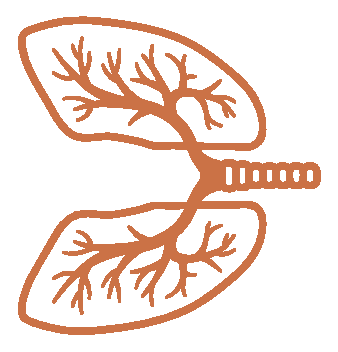
\includegraphics[scale=0.6]{lung}};
 \node[above]at(LUNG.north){Patient};
%
\begin{scope}[on background layer]
\draw[draw=none,
fill=cyan!10]([xshift=-25,yshift=-6]VE2)coordinate(PB1)
--++(0:2.25)coordinate(PB2)
--++(0:7.0)coordinate(PB3)
--++(270:3.2)coordinate(PB4)
--++(180:7.0)coordinate(PB5)
--++(180:2.25)coordinate(PB6)
--cycle;
%
\draw[line width=1pt,black!40,
dashed](PB1)--(PB3)
(PB2)--(PB5)
(PB1)--(PB6);
\end{scope}
\end{tikzpicture}
\end{document}
